\documentclass[tikz]{standalone}
%\usetikzlibrary{...}% tikz package already loaded by 'tikz' option
    \newcommand{\point}[1]{\draw[shift=#1,fill=black] (0,0) circle (.1);}
\newcommand{\HP}[1]{
    % base
    \draw[thick] (3.4,1) ellipse (.6 and 1);
    \draw[thick] (.6,0) -- (3.4,0);
    \draw[thick] (.6,2) -- (3.4,2);
    \begin{scope}
        \clip (-1,-.2) rectangle (.6,2.2) ;
        \draw[thick] (.6,1) ellipse (.6 and 1);
    \end{scope}

    % numero
    \draw (3.4,0) node[above,scale=4] {#1};

    % bornes
    \draw[fill=black] (1,1) circle (.2) node[above right, scale=2] {+};
    \draw[thick] (2,1) circle (.2) node[above right, scale=2] {-};
}
\newcommand{\baseHP}{
    % 4 sources
    \begin{scope}[shift={(0,0)}] \HP{1} \end{scope}
    \begin{scope}[shift={(5,0)}] \HP{2} \end{scope}
    \begin{scope}[shift={(0,-3)}] \HP{3} \end{scope}
    \begin{scope}[shift={(5,-3)}] \HP{4} \end{scope}

    %  +/- généraux
    \draw[fill=black] (-3,-.5) circle (.2) ++(-.3,0) node[left, scale=2] {+};
    \draw[thick] (-3,-1) circle (.2) ++(-.3,0) node[left, scale=2] {-};
}


\begin{document}
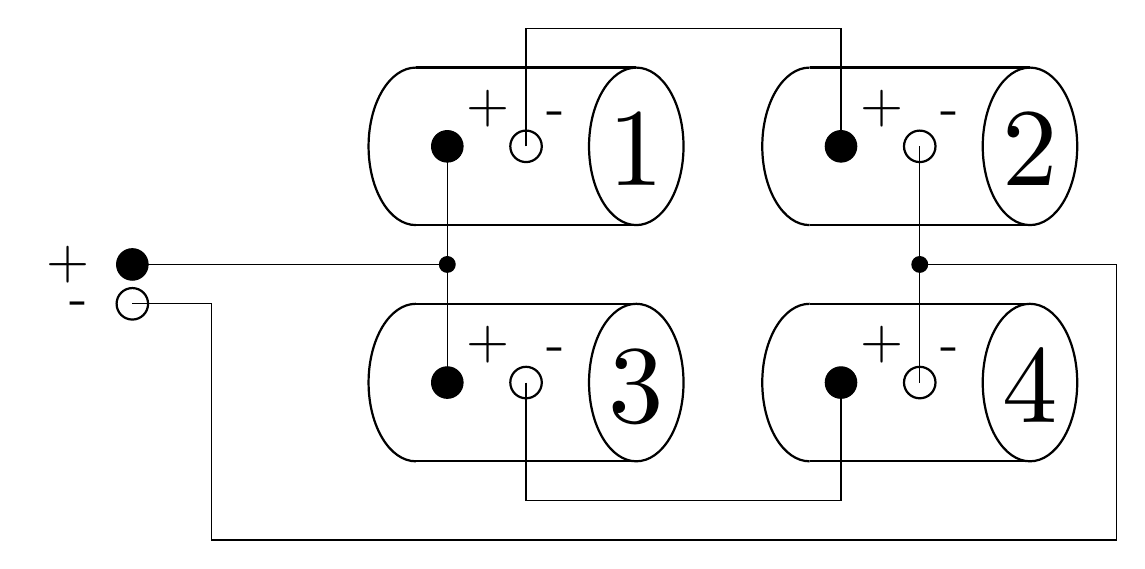
\begin{tikzpicture}% Example:
    % grille de dessin
    % \draw[red] (-10,-10) grid (10, 10);

    \baseHP

    % +
    \draw (-3,-.5) -- (1,-.5);
    \draw (1,1) -- (1,-2);
    \point{{(1,-.5)}}

    % bondings
    \draw (2,1) -- (2,2.5) -- (6,2.5) -- (6,1);
    \draw (2,-2) -- (2,-3.5) -- (6,-3.5) -- (6,-2);

    % -
    \draw (-3,-1) -- (-2,-1) -- (-2,-4) -- (9.5,-4) -- (9.5,-.5) -- (7, -.5);
    \draw (7,1) -- (7,-2);
    \point{{(7,-.5)}}



\end{tikzpicture}
\end{document}
